\documentclass[12pt]{article}
\usepackage{cite}
\usepackage{graphicx}
\usepackage{geometry}
\usepackage{float}
\usepackage{multicol}

\geometry{left=2.0cm,right=2.0cm,top=2.5cm,bottom=2.5cm}

\title{
    \textbf{\Huge ECE385} \\
    \huge Fall 2020 \\
    \huge Experiment 4 \\[120pt]
    \textbf{\Huge Introduction to SystemVerilog, FPGA, CAD and 16-bit Adders} \\[120pt]
    }

\author{
    \large Name: Zhou Qinren \\ 
            \quad\qquad Zhang Yichi \\
    \large Lab Section: LA3 \\
    \large TA's Name: Yu Yuqi
    }

\date{Oct. $19^{th}$ 2020}

\begin{document}
\setlength{\parindent}{0pt}
\maketitle
\newpage

\section{Introduction}
The serial logic processor performs the same function as in Lab 3, except we extend the register to 8-bit. The processor takes in two inputs and performs a particular function according to the F2F1F0 signal.

The three adders realize the addition of two 16 bits addends, but they differ in performance. The ripple adder is the simplest, but the slowest. The CLA and CSA are faster, but more complicated. 


\section{Serial Logic Processor}
\subsection{block diagram}
\begin{figure}[H]
    \centering
    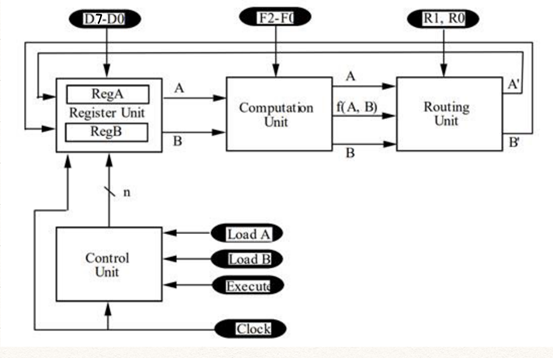
\includegraphics{toplevel_block_diagram.png}
    \caption{Top level block diagram.}
\end{figure}

\begin{figure}[H]
    \centering
    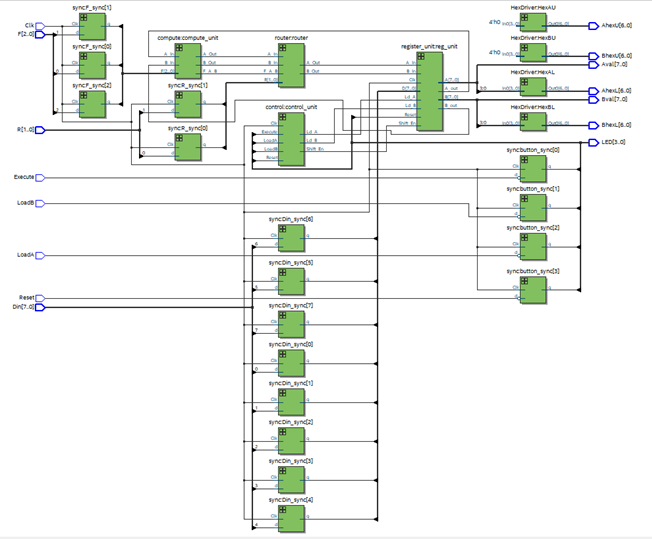
\includegraphics{toplevel_RTL.png}
    \caption{Top level RTL diagram.}
\end{figure}
\subsection{To extend the processor from 4 bits to 8 bits}
1. Modify the reg4 unit, extend it to 8 bits. Find out the code involving register size and change it. \\

2. Modify the register unit, since it makes use of two 4-bit register in before. Change it to 8-bit registers. \\

3. Modify the processor. Both the data input and output signals should be extended to 8 bits. Modify the local variable that involves the content of the register unit. Add more Hex driver, since we are using two 8-bit register. Modify the state machine so as to extend the running cycles to 8 instead of 4.

\begin{figure}[H]
    \centering
    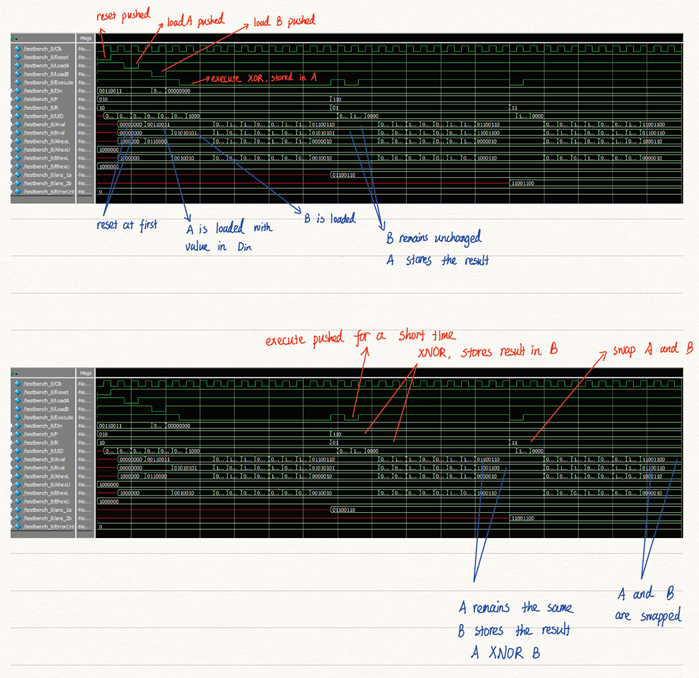
\includegraphics{processor_simulation.png}
    \caption{Simulation of 8-bit processor.}
\end{figure}

\section{Adders}
\subsection{Ripple Carry Adder (CRA)}
16-bit CRA consists of three hierarchies. \\

The bottom hierarchy is a full adder which computes 1 bit numbers and outputs the result and the carry out. \\

\begin{figure}[H]
    \centering
    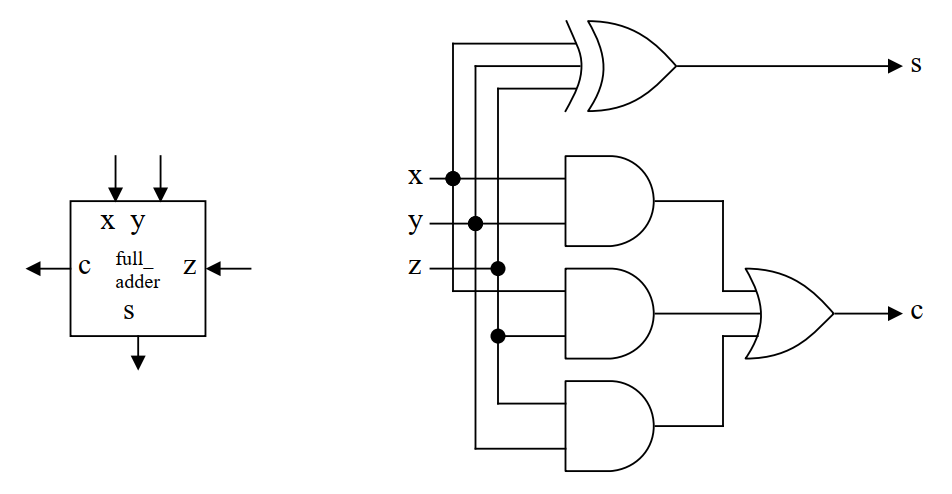
\includegraphics[width=15cm]{full_adder.png}
    \caption{Full adder block diagram \cite{GG4.3}}
\end{figure}

The middle hierarchy, four-bit CRA, is composed of 4 full adders in sequence which computes 4 bits numbers and outputs the result and the carry out. \\

The top hierarchy, is comprised of 4 four-bit CRA in sequence which computes 16 bits numbers and outputs the result and the carry out.

\begin{figure}[H]
    \centering
    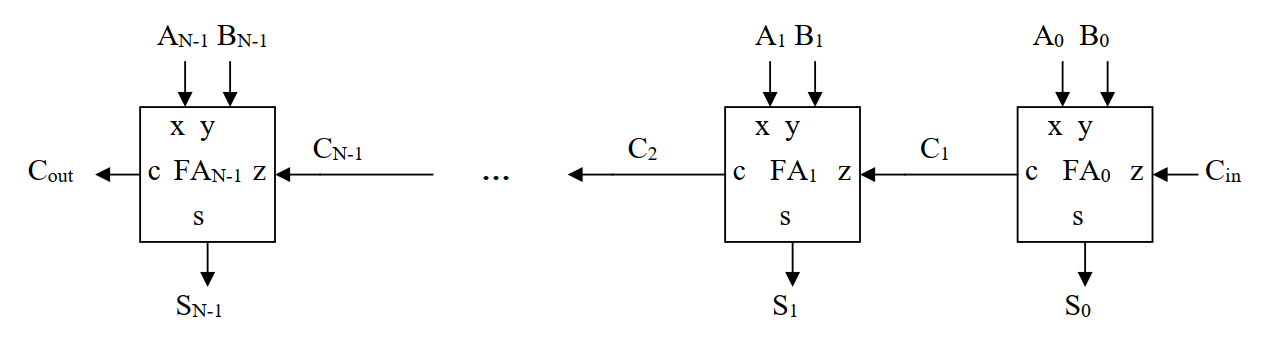
\includegraphics[width=18cm]{N_bit_CRA.png}
    \caption{N-bit CRA block diagram. $N=4$ for the middle hierarchy four-bit CRA. $N=16$ for the top hierarchy 16-bit CRA. \cite{GG4.3}}
\end{figure}

\subsection{Carry Lookahead Adder (CLA)}
CLA uses the concept of generating (G) and propagating (P). $G=A \cdot B$ means that there must be a carry out 1 regardless of the carry in. $P=A \oplus B$ means that only one of the A and B is 1 so the carry out is decided by the carry in. Therefore, all the carry in $C_1$ to $C_16$ (cout) can be expressed by G, P and $C_0$ (cin), $C_{i+1}=G_i+(P_i \cdot C_i)$.\\

16-bit CLA consists of three hierarchies. \\

The bottom hierarchy is also a full adder which computes 1 bit numbers and outputs the result. \\

The middle hierarchy, four-bit CLA, is composed of 4 full adders which computes 4 bits numbers and outputs the result. In this module, $p[3:0]$ and $g[3:0]$ can be directly calculated by $A[3:0]$ and $B[3:0]$ and therefore so do the $cin[3:0]$. Thus, the 4 full adders do not need to wait for the former one to provide cin and can start working as long as the cin is calculated. \\

\begin{figure}[H]
    \centering
    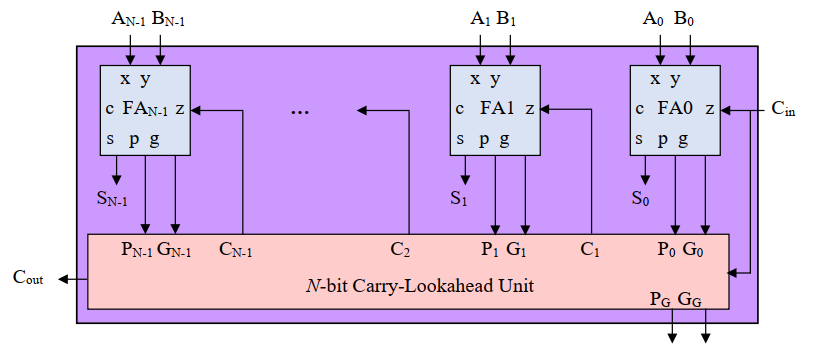
\includegraphics[width=15cm]{N_bit_CLA.png}
    \caption{N-bit CLA block diagram. For the middle hierarchy four-bit CLA, $N=4$ here. \cite{GG4.4}}
\end{figure}

\begin{figure}[H]
    \centering
    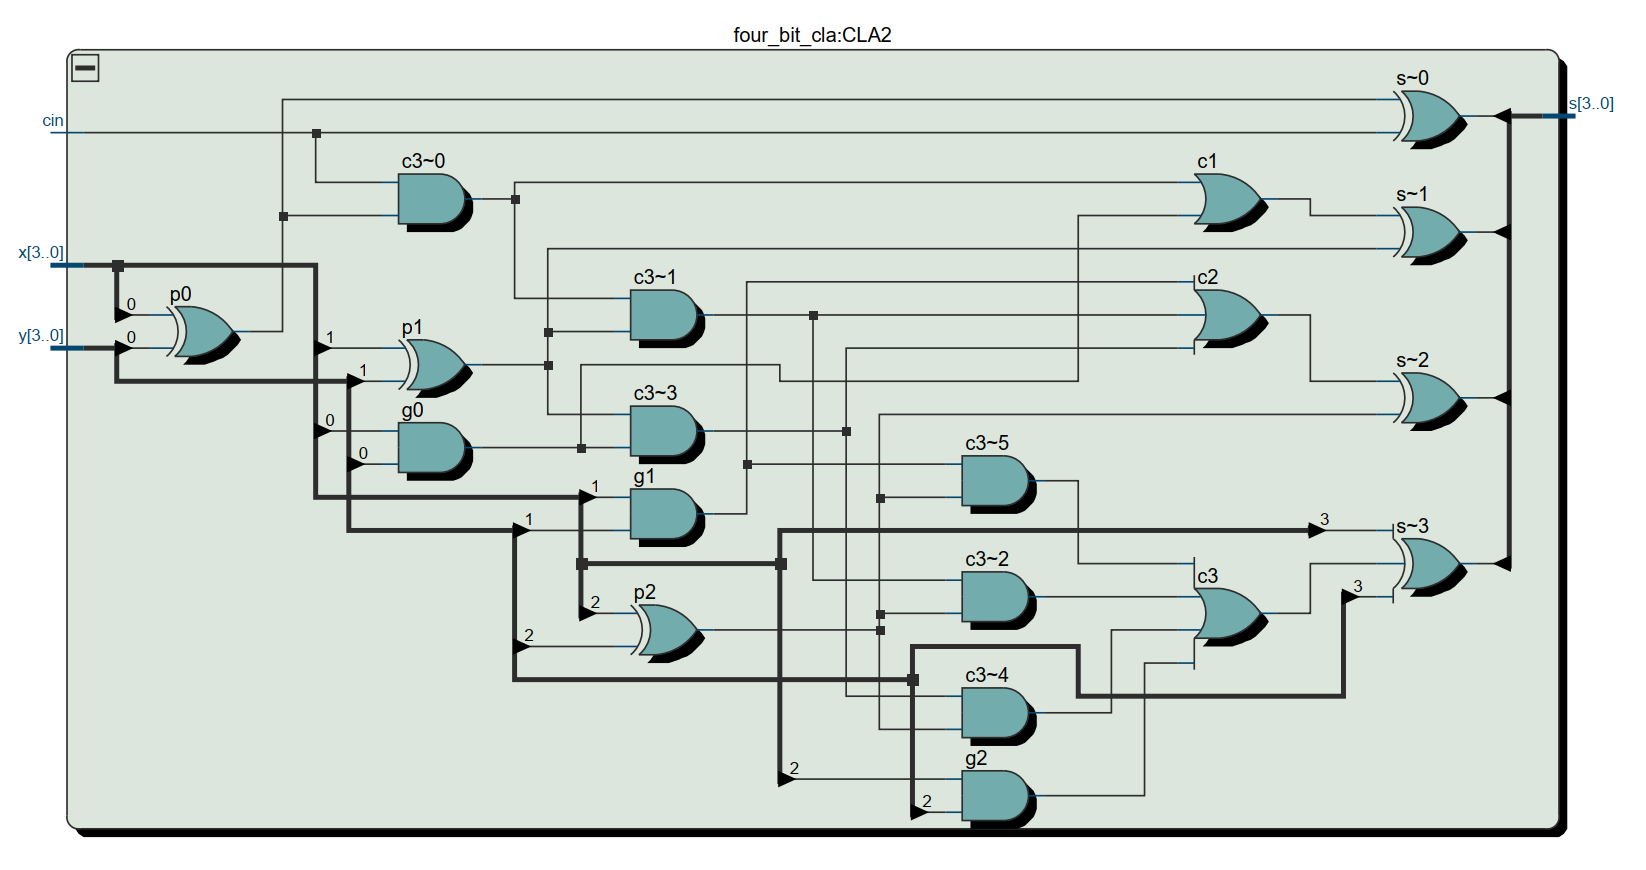
\includegraphics[width=15cm]{CLA_4bit.png}
    \caption{4-bit CLA RTL diagram.}
\end{figure}

The top hierarchy, is comprised of 4 four-bit CLAs which computes 16 bits numbers and outputs the result and the carry out. Similar to the four-bit CLA, $p[15:0]$ and $g[15:0]$ can be directly calculated by $A[15:0]$ and $B[15:0]$. We form 4 ps to be one group $pg=p0 \cdot p1 \cdot p2 \cdot p3$ and 4 gs to be one group $gg=g3+g2 \cdot p3+g1 \cdot p3 \cdot p2+g0 \cdot p3 \cdot p2 \cdot p1$. After that, we will have 4 new pgs and ggs. With the same formula, $C_{i+1}=G_i+(P_i \cdot C_i)$, we can calculate $C_4$, $C_8$, $C_{12}$ as 3 cin for the four-bit CLAs and $C_{16}$ as the carry out. Consequently, the 4 four-bit CLAs do not need to wait for the former one to provide cin and can start working as cins have already been calculated.

\begin{figure}[H]
    \centering
    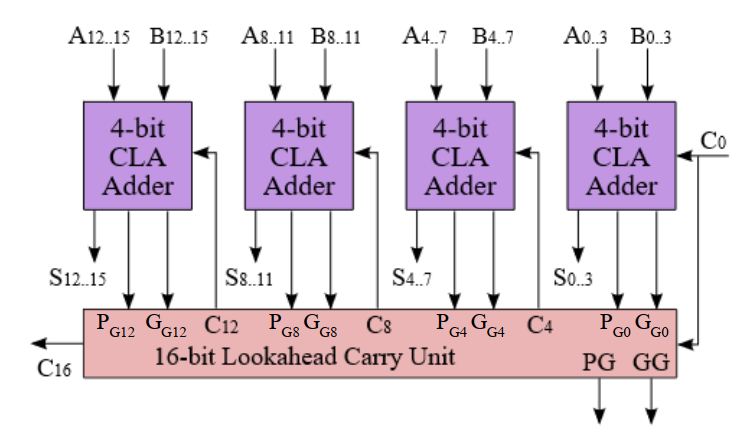
\includegraphics[width=12cm]{4x4_CLA.png}
    \caption{4x4-bit hierarchical CLA block diagram for the top hierarchy. \cite{GG4.6}}
\end{figure}

\begin{figure}[H]
    \centering
    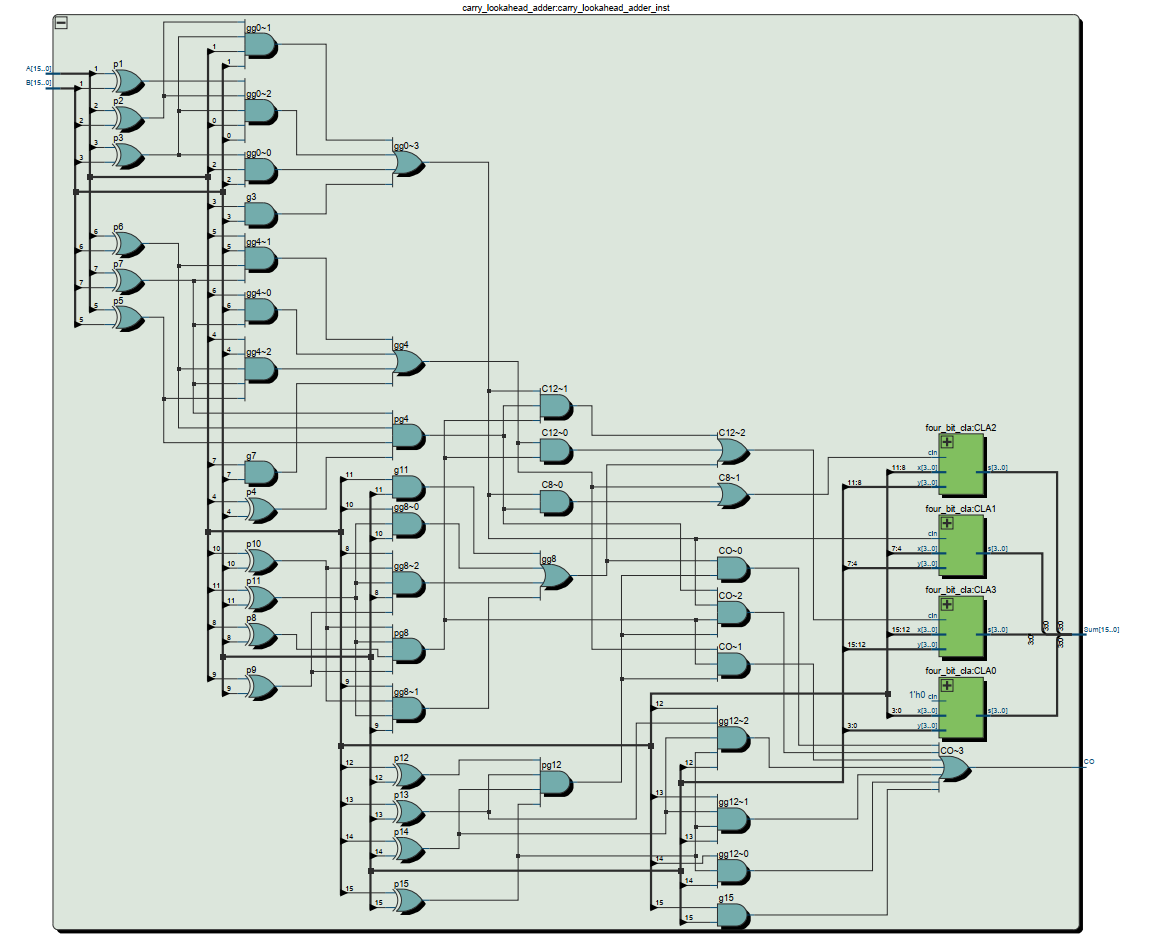
\includegraphics[width=15cm]{CLA_top.png}
    \caption{4x4-bit hierarchical CLA RTL diagram.}
\end{figure}

\subsection{Carry Select Adder}
16-bit CLA consists of three hierarchies. The bottom and middle hierarchies are exactly the same as the CRA's. \\

The top hierarchy is comprised of 7 four-bit CRAs which computes 16 bits numbers and outputs the result and the carry out. 7 four-bit CRAs calculates all the possibilities - $C_4,C_8,C_{12}=0$, $C_4,C_8,C_{12}=1$ and $C_0=cin$ - simultaneously since all the cins are given. Then, we use a mux and the cout of the former CRAs to decide the next cout and the final result.

\begin{figure}[H]
    \centering
    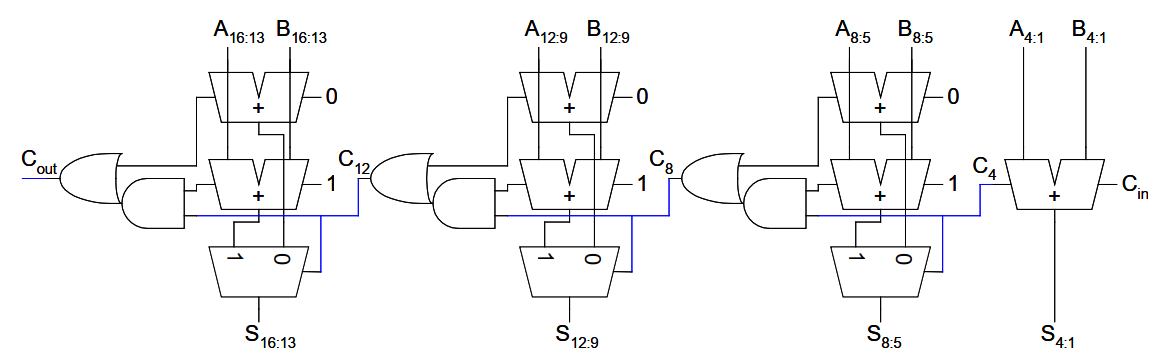
\includegraphics[width=15cm]{16_bit_CSA.png}
    \caption{16-bit CSA block diagram for the top hierarchy. \cite{GG4.6}}
\end{figure}

\begin{figure}[H]
    \centering
    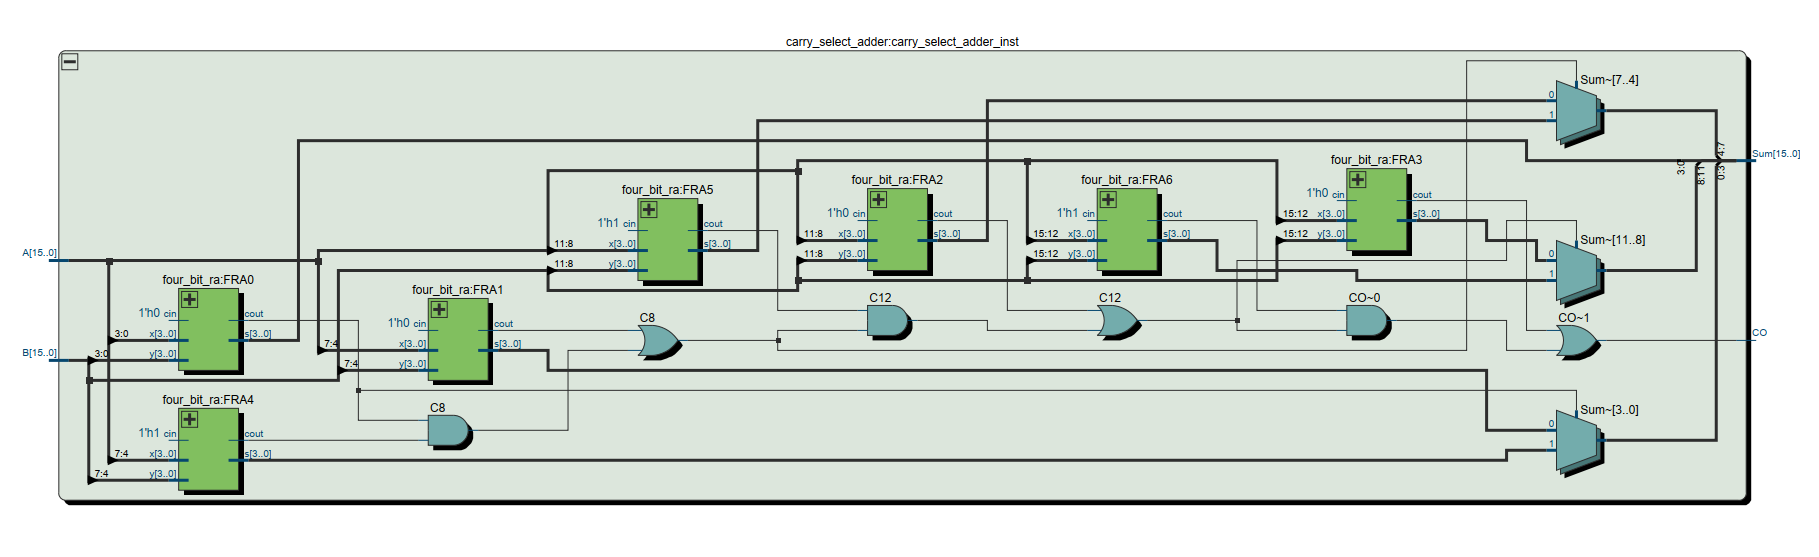
\includegraphics[width=18cm]{CSA_RTL.png}
    \caption{16-bit CSA RTL diagram for the top hierarchy.}
\end{figure}

\subsection{Written Description of All .sv Modules}
\begin{table}[H]
    \begin{tabular}{|l|}

    \hline
    \begin{tabular}{p{1\columnwidth}}
        \textbf{Module}: full adder \\ 
        \textbf{Inputs}: x, y, cin \\ 
        \textbf{Outputs}: s, cout \\ 
        \textbf{Description}: Calculate $x+y+cin$, store the result in $s$ and the carry out bit in $cout$.\\ 
        \textbf{Purpose}: This is a 1-bit adder serving as the bottom hierarchy for all the N-bit adders.
    \end{tabular} \\
    \hline

    \hline
    \begin{tabular}{p{1\columnwidth}}
        \textbf{Module}: four bit ra \\ 
        \textbf{Inputs}: [3:0] x, [3:0] y, cin \\ 
        \textbf{Outputs}: [3:0] s, cout \\ 
        \textbf{Description}: Call full adder module four times to calculate $x+y+cin$. Store the result in $s$ and the carry out bit in $cout$. \\ 
        \textbf{Purpose}: This is a four-bit CRA.
    \end{tabular} \\
    \hline

    \hline
    \begin{tabular}{p{1\columnwidth}}
        \textbf{Module}: ripple adder\\ 
        \textbf{Inputs}: [15:0] A, [15:0] B \\ 
        \textbf{Outputs}: [15:0] Sum, CO \\ 
        \textbf{Description}: Call four bit ra module four times to calculate $A+B$. Store the result in $Sum$ and the carry out bit in $CO$. \\ 
        \textbf{Purpose}: This is a 16-bit CRA.
    \end{tabular} \\
    \hline

    \hline
    \begin{tabular}{p{1\columnwidth}}
        \textbf{Module}: four bit cla \\ 
        \textbf{Inputs}: [3:0] x, [3:0] y, cin \\ 
        \textbf{Outputs}: [3:0] s \\ 
        \textbf{Description}: Calculate g[3:0], p[3:0] and c[3:0] by $g_i=x_i \cdot y_i$ and $p_i=x_i \oplus y_i$, $c_{i+1}=g_i+(p_i \cdot c_i)$ and $c_0=cin$. With all the cin then calculate s[3:0]. \\ 
        \textbf{Purpose}: This is a four-bit CLA which will be the basis for 16-bit CLA.
    \end{tabular} \\
    \hline
    
    \hline
    \begin{tabular}{p{1\columnwidth}}
        \textbf{Module}: carry lookahead adder \\ 
        \textbf{Inputs}: [15:0] A, [15:0] B \\ 
        \textbf{Outputs}: [15:0] Sum, CO \\ 
        \textbf{Description}: Calculate g[15:0], p[15:0] and c[15:0] by $g_i=x_i \cdot y_i$ and $p_i=x_i \oplus y_i$, $c_{i+1}=g_i+(p_i \cdot c_i)$ and $c_0=0$. With all the cins, call the four bit cla 4 times to let them run simultaneously. \\ 
        \textbf{Purpose}: This is a 16-bit CLA.
    \end{tabular} \\
    \hline

    \hline
    \begin{tabular}{p{1\columnwidth}}
        \textbf{Module}: carry select adder \\ 
        \textbf{Inputs}: [15:0] A, [15:0] B \\ 
        \textbf{Outputs}: [15:0] Sum, CO \\ 
        \textbf{Description}: Call the four bit ra 7 times to calculate $A[3 : 0]+B[3 : 0]$, $A[7 : 4]+B[7 : 4]$, $A[11: 8]+B[11: 8]$, $A[15:12]+B[15:12]$ with $cin=0$ and $A[7 : 4]+B[7 : 4]$, $A[11: 8]+B[11: 8]$, $A[15:12]+B[15:12]$ with $cin=1$. Then use C4 to select Sum[7:4] and C8, use C8 to select Sum[11:8] and C12 then use C12 to select Sum[15:12] and C16 (CO).\\ 
        \textbf{Purpose}: This is a 16-bit CSA.
    \end{tabular} \\
    \hline

    \hline
    \begin{tabular}{p{1\columnwidth}}
        \textbf{Module}: HexDriver \\ 
        \textbf{Inputs}: [3:0] In0\\ 
        \textbf{Outputs}: [6:0] Out0\\ 
        \textbf{Description}: The HexDriver module takes in a 4-bit number and outputs its corresponding 7-bit number representing a hex number (one of "0123456789ABCDEF"). \\ 
        \textbf{Purpose}: HexDriver turns the result 4-bit number to its corresponding hex number for FPGA to show on the digital monitor.
    \end{tabular} \\
    \hline

    \end{tabular}
\end{table}

\subsection{Area, Complexity, and Performance Tradeoffs}
For the area, we consider the LUT used by each adder. CLA uses up the most area, while the CRA uses up the least area. For the complexity, we consider the difficulty of the design. CRA and CSA are both very easy to design. CLA has the most complexity. For the performance, we consider the frequency. The higher the frequency is, the better the performance is. Therefore, CSA has the best performance. CLA is the next. CRA has the worst performance. As for the tradeoffs, CLA and CSA have better performance but consumes more energy and uses up more areas.

\subsection{Performance Graph}
\begin{figure}[H]
    \centering
    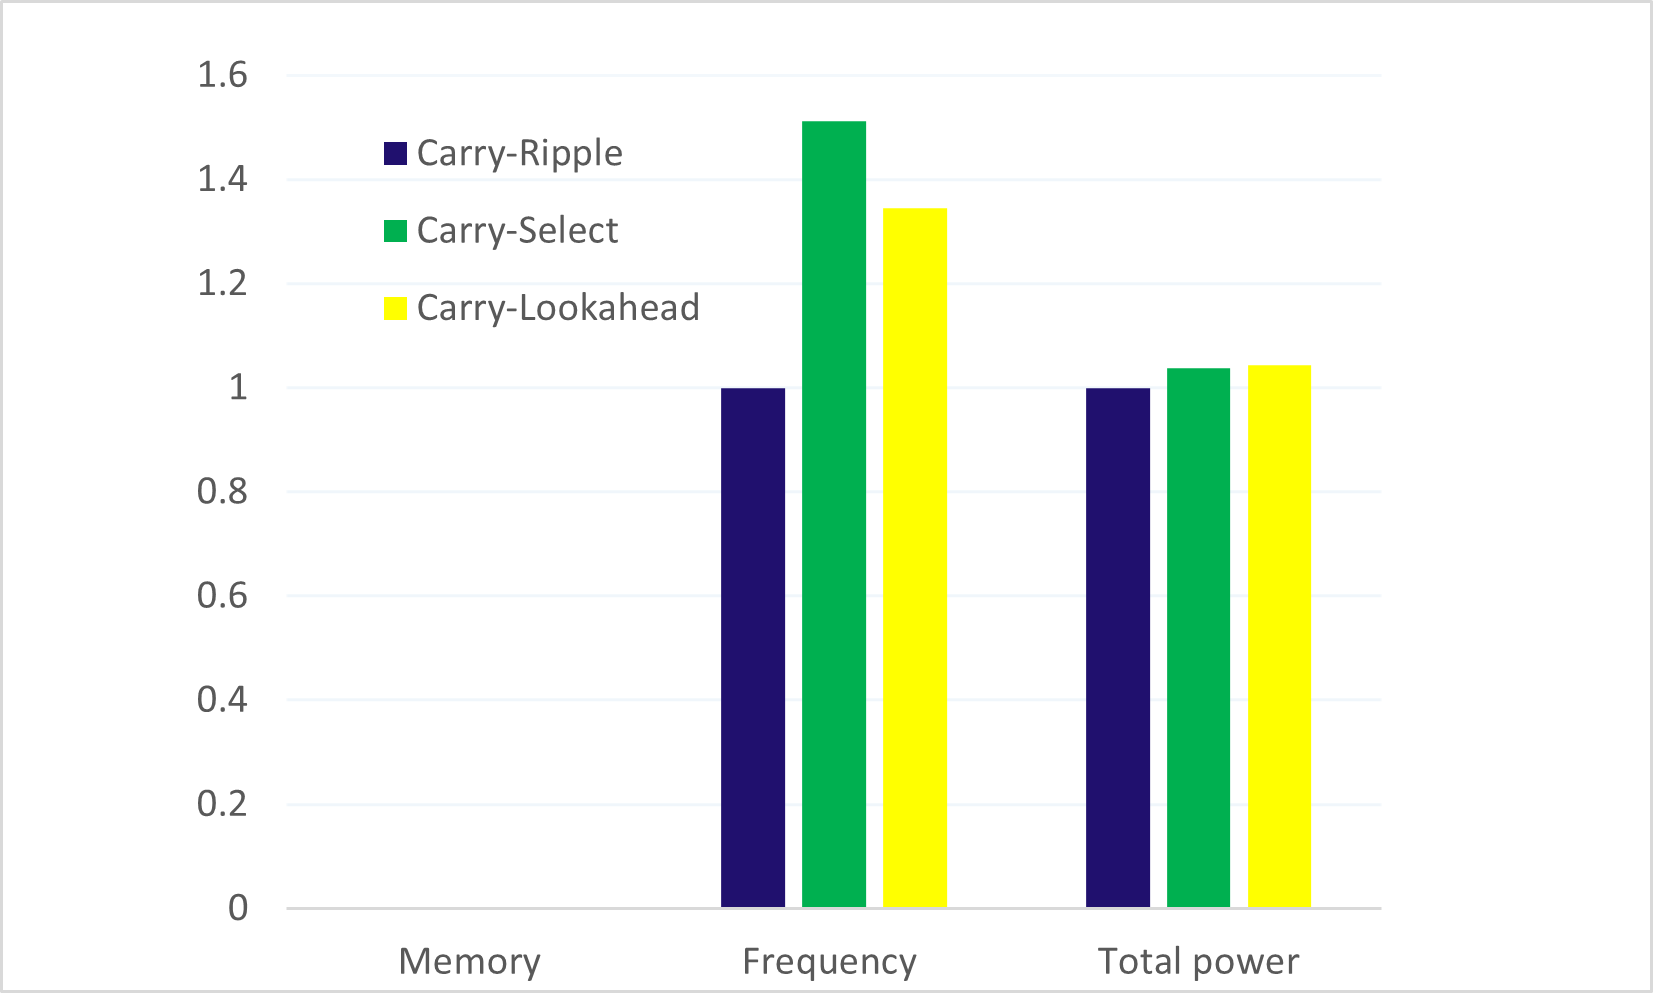
\includegraphics{prelab.png}
    \caption{Performance graph.}
\end{figure}

\section{Answers to Pre-Lab and Post-Lab Questions}
Question: Compare the usage of LUT, Memory, and Flip-Flop of your bit-serial logic processor exercise in the IQT with your TTL design in Lab 3. Make an educated guess of the usage of these resources for TTL assuming the processor is extended to 8-bit. Which design is better, and why? \\

Answer: The 4-bit logic processor in lab4 exercise uses 46 LUTs, 0 memory and 27 flip-flops. The TTL design in lab3 requires 22 LUTs, 0 memory and 12 flip-flops. \\
The 8-bit logic processor in lab4 uses 58 LUTs, 0 memory and 63 flip-flops. If the TTL design is extended to 8 bits, we expect it to use 34 LUTs, 0 memory and 20 flip-flops. \\
TTL design is better in performance, since it requires less logic element, and the logic is simpler, therefore, faster. However, the development is time-consuming, and bugs appear more often. \\

Question: In the CSA for this lab, we asked you to create a 4x4 hierarchy. Is this ideal? \\

Answer: Ideal. \\

Question: Complete the following design statistics table for each adder. Observe the data plot and provide explanation to the data. 

\begin{table}[H]
    \centering
    \resizebox*{12cm}{6cm}{
        \begin{tabular}{|l|l|l|l|}
        \hline
        Adders        & CRA      & CLA      & CSA      \\ \hline
        LUT           & 114      & 131      & 123      \\ \hline
        DSP           & 0        & 0        & 0        \\ \hline
        Memory        & 0        & 0        & 0        \\ \hline
        Flip-Flop     & 105      & 105      & 105      \\ \hline
        Frequency     & 62.73MHz & 84.38MHz & 94.89MHz \\ \hline
        Static Power  & 98.55mW  & 98.57mW  & 98.56mW  \\ \hline
        Dynamic Power & 3.07mW   & 6.84mW   & 6.28mW   \\ \hline
        Total Power   & 155.93mW & 162.52mW & 161.65mW \\ \hline
        \end{tabular}
    }
    \caption{Design statistics table for CRA, CLA and CSA.}
\end{table}

LUT: the number of look up tables. \\
DSP: not used for this lab. \\
BRAM: not used for this lab. \\
Flip-flop: the number of registers. \\

The data makes sense. CRA is the simplest, and CLA is the most complicated, because of the logic for Ps and Gs. \\
CSA has the largest Fmax, CLA has the second, and CRA has the least. This also fits our expectation, because CSA runs addition parallelly of every 4 bits, while CLA has to calculate the carry-in logic, which becomes extremely complicated for P, G of most significant bits. CRA has to run in sequential order, therefore, it is the slowest. \\
CRA has the least power consumption, since its logic is simple. CSA and CLA has almost the same power consumption, which is a little out of our expectation. We expect CLA to have a larger power, since it is much more complicated than CSA. The reason might be our design size is too small, the difference is therefore insignificant. 


\section{Conclusion}
\subsection{Bugs Encountered}
During design process, we occasionally drive more than one constant values to one variable. To avoid this, we use two or more local variables, and connect these two variables with the original one, and add some if-else logic, in which case we create a mux.

\subsection{About the Lab Manual}
As we are asked to answer the questions about the performance (e.g. LUT, LE, area, frequency, etc.), we are looking forward to seeing more clear definition and analysis examples in the lab manual. Also, more SystemVerilog instructions are welcome.

\subsection{Additional Summary}
We have learnt how to write modules, instantiate and connect them in the top-level entity to establish a project. We also get familiar with the idea that the code in HDL runs concurrently, which is different from software language. 

\newpage
\bibliography{lab4_ref}
\bibliographystyle{ieeetr}
\end{document}